\documentclass{article}
\usepackage[utf8]{inputenc}
\usepackage[portuguese]{babel}
\usepackage{csquotes}
\usepackage{graphicx}
\usepackage{adjustbox}
\usepackage{lipsum}
\usepackage[backend=biber,autolang=other,
  bibencoding=utf8,style=alphabetic,
  ibidtracker=true]{biblatex}
\addbibresource{polo-natural.bib}

\title{Franscisco d'Holanda e o Tirar Pelo Natural} \date{2 de
  Julho de 2015} \author{João Távora \\Faculdade de Belas Artes da
  Universidade de Lisboa}

\begin{document}

\maketitle

\section{Sinopse}

``Do Tirar Polo Natural'' é uma  de Francisco
d'Holanda (1517 – 1585), arquitecto, ilustrador, humanista, ensaísta e
figura chave da Renascença Portuguesa. 

\section{Palavras-chave}

Francisco d'Holanda, Desenho, Retrato

\section{Introdução}

\section{Aspectos biográficos}

O prólogo d'``[o] Tirar Pelo Natural'' é fértil em indícios
biográficos sobre Francisco de Holanda. Segundo o autor, foi numa
particular etapa de uma viagem a Santiago de Compostela com o infante
D. Luís, que se proporcionou uma paragem no Porto, onde o tomou por
hóspede Braz Pereira, filho de Fernando Brandão, antigo fidalgo ao
serviço do infante D. Fernando. F. d'H. explica como terá sido durante
a infância criado com Braz Pereira, e que lhe foi fácil aceitar a
oferta de hospitalidade.

O autor declara que a estada em casa de Braz Pereira é frequente, e
como lhes é costume discutir pintura e arquitectura nessas ocasiões,
``gastando nisso parte das noites'', mas insiste em clarificar que
nesta ocasião é uma encomenda do próprio infante D. Luís, de quem se
aparta em Amarante, de que através de uns intermediários, se
entregassem a Braz Pereira umas cabeças de gesso antigas provindas de
Roma, para que finalmente pudessem estas ser expedidas para Lisboa por
via marítima.

E é nessa estadia de ``oito dias, de vida boa'' em casa de Braz
Pereira, que se produz segundo F. d'H o desejo de registar as
observações que ali se produziam sobre pintura ao natural. E
declarando o autor que ``será melhor ouvir o que cada um dizia nesta
prática que perder-se mais o tempo''\cite[p12]{holanda}, justifica
desta forma a escolha da forma do diálogo para o livro.

TODO: Amarante
TODO: Porto cidade estrangeira em Portugal

\section{A relação com o modelo}

``singular''\cite[pxx]{holanda}:

\begin{quote}
\end{quote}

\section{Os mestres singulares}

\section{Conclusão}

A escolha da forma de diálogo para o livro, extensamente justificada
no prólogo com pormenores anedóticos de duvidosa relevância, é um
claríssimo piscar de olho às obras do próprio Platão, com
F. d'H. despreocupadamente a tomar o lugar do sofista Sócrates e Braz
Pereira o lugar de aprendiz.

TODO:  Tomava-se em grande conta.

lorem lorem lorem lorem lorem lorem lorem lorem lorem lorem lorem
lorem lorem lorem lorem lorem lorem lorem lorem lorem lorem lorem
lorem lorem lorem lorem lorem lorem

\begin{figure}
\centering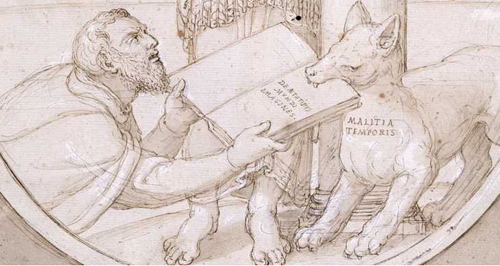
\includegraphics[height=0.3\textheight,keepaspectratio]
                          {images/malatia-temporis.png}
  \caption{Pormenor de um desenho de Franscisco da Holanda, ``O
    artista apresentando o seu livro''}
  \label{fig:1}
\end{figure}

lorem lorem lorem lorem lorem lorem lorem lorem lorem lorem lorem
lorem lorem lorem lorem lorem lorem lorem lorem lorem lorem lorem
lorem lorem lorem lorem lorem lorem

\printbibliography[heading=bibliography,title={Bibliografia}]

\end{document}
